\documentclass{standalone}
\usepackage{tikz-network}

\begin{document}
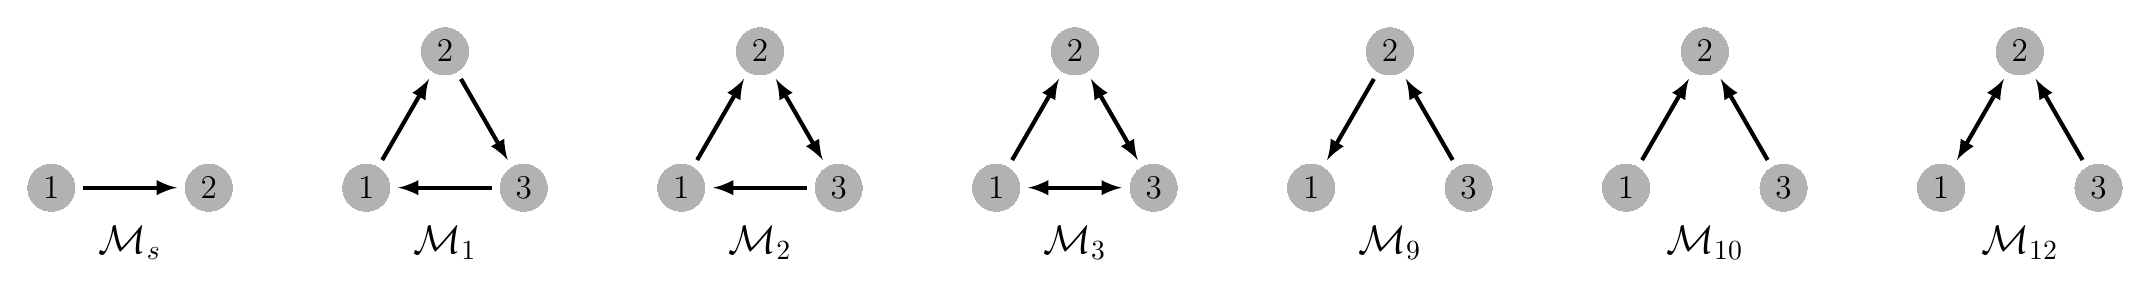
\begin{tikzpicture}

\SetVertexStyle[LineWidth=0, FillColor=black!30!white, LineColor=black!30!white, OuterSep=3, TextFont=\large]
\SetEdgeStyle[Color=black]
\SetTextStyle[TextFont=\Large]

\Vertex[x=-4,label=1]{Ma_1}
\Vertex[x=-2,label=2]{Ma_2}
\Edge[Direct](Ma_1)(Ma_2)
\Text[x=-3,y=-0.7]{$\mathcal{M}_s$}

\Vertex[x=0,label=1]{M1_1}
\Vertex[x=1,y=1.732,label=2]{M1_2}
\Vertex[x=2,label=3]{M1_3}
\Edge[Direct](M1_1)(M1_2)
\Edge[Direct](M1_2)(M1_3)
\Edge[Direct](M1_3)(M1_1)
\Text[x=1,y=-0.7]{$\mathcal{M}_1$}

\Vertex[x=4,label=1]{M2_1}
\Vertex[x=5,y=1.732,label=2]{M2_2}
\Vertex[x=6,label=3]{M2_3}
\Edge[Direct](M2_1)(M2_2)
\Edge[Direct,style=latex-latex](M2_2)(M2_3)
\Edge[Direct](M2_3)(M2_1)
\Text[x=5,y=-0.7]{$\mathcal{M}_2$}

\Vertex[x=8,label=1]{M3_1}
\Vertex[x=9,y=1.732,label=2]{M3_2}
\Vertex[x=10,label=3]{M3_3}
\Edge[Direct](M3_1)(M3_2)
\Edge[Direct,style=latex-latex](M3_2)(M3_3)
\Edge[Direct,style=latex-latex](M3_3)(M3_1)
\Text[x=9,y=-0.7]{$\mathcal{M}_3$}

\Vertex[x=12,label=1]{M9_1}
\Vertex[x=13,y=1.732,label=2]{M9_2}
\Vertex[x=14,label=3]{M9_3}
\Edge[Direct](M9_3)(M9_2)
\Edge[Direct](M9_2)(M9_1)
\Text[x=13,y=-0.7]{$\mathcal{M}_9$}

\Vertex[x=16,label=1]{M10_1}
\Vertex[x=17,y=1.732,label=2]{M10_2}
\Vertex[x=18,label=3]{M10_3}
\Edge[Direct](M10_1)(M10_2)
\Edge[Direct](M10_3)(M10_2)
\Text[x=17,y=-0.7]{$\mathcal{M}_{10}$}

\Vertex[x=20,label=1]{M12_1}
\Vertex[x=21,y=1.732,label=2]{M12_2}
\Vertex[x=22,label=3]{M12_3}
\Edge[Direct, style=latex-latex](M12_1)(M12_2)
\Edge[Direct](M12_3)(M12_2)
\Text[x=21,y=-0.7]{$\mathcal{M}_{12}$}


\end{tikzpicture}
\end{document}